%!TEX encoding = UTF-8 Unicode

\documentclass[a4paper]{article}

\usepackage{INTERSPEECH_v2}

\usepackage[T1]{fontenc} % output - specifies encoding used in fonts; needs full LaTeX distribution to produce good-looking output
\usepackage[utf8]{inputenc} % input - type accented characters directly from keyboard
\usepackage[english]{babel} % internationalization - hyphenation, typographic rules for one or more languages

\usepackage[nolist]{acronym}
\usepackage{amsmath}
\usepackage{amssymb}
%\usepackage{epigraph}
\usepackage{hyperref}
\graphicspath{{figures/}}

\title{Interactive Robot Learning of Gestures, Language and Affordances}
\name{Giovanni~Saponaro$^1$, Giampiero~Salvi$^2$, Lorenzo~Jamone$^{3,1}$, Alexandre~Bernardino$^1$}
\address{
  $^1$Institute for Systems and Robotics\\Instituto Superior Técnico, Universidade de Lisboa, Lisbon, Portugal\\
  $^2$KTH Royal Institute of Technology, Stockholm, Sweden\\
  $^3$ARQ~(Advanced Robotics at Queen Mary)\\School of Electronic Engineering and Computer Science, Queen Mary University of London, UK}
\email{gsaponaro@isr.tecnico.ulisboa.pt, giampi@kth.se, l.jamone@qmul.ac.uk, alex@isr.tecnico.ulisboa.pt}

% custom commands and frequent expressions that require typesetting care
\newcommand{\eg}{e.\,g.}
\newcommand{\ie}{i.\,e.}
\newcommand{\HR}{Human--Robot}
\newcommand{\HRI}{\HR{} Interaction}
\newcommand{\hh}{human--human}
\newcommand{\hr}{human--robot}
\newcommand{\hri}{\hr{} interaction}

% examples and useful stuff from INTERSPEECH template

% \begin{table}
%   \caption{This is an example of a table}
%   \label{tab:example}
%   \centering
%   \begin{tabular}{ r@{}l  r }
%     \toprule
%     \multicolumn{2}{c}{\textbf{Ratio}} &
%                                          \multicolumn{1}{c}{\textbf{Decibels}} \\
%     \midrule
%     $1$                       & $/10$ & $-20$~~~             \\
%     $1$                       & $/1$  & $0$~~~               \\
%     $2$                       & $/1$  & $\approx 6$~~~       \\
%     $3.16$                    & $/1$  & $10$~~~              \\
%     $10$                      & $/1$  & $20$~~~              \\
%     $100$                     & $/1$  & $40$~~~              \\
%     $1000$                    & $/1$  & $60$~~~              \\
%     \bottomrule
%   \end{tabular}
% \end{table}

%\begin{figure}
%  \centering
%  \includegraphics[width=\linewidth]{figure.pdf}
%  \caption{Schematic diagram of speech production.}
%  \label{fig:speech_production}
%\end{figure}

% For technical reasons, the proceedings editor will strip all active links from the papers during processing. Hyperlinks can be included in your paper, if written in full, e.\,g.\ ``http://www.foo.com/index.html''. The link text must be all black.
% Please make sure that they present no problems in printing to paper.

% list of acronyms
\begin{acronym}
\acro{BN}{Bayesian Network}
\acro{HMM}{Hidden Markov Model}
\acro{MTRNN}{Multiple Timescales Recurrent Neural Network}
\end{acronym}

\begin{document}

\maketitle
%
\begin{abstract} % max 200 words
  blah
\end{abstract}
\noindent\textbf{Index Terms}: cognitive robotics, gesture recognition, object affordances

%%%%%%%%%%%%%%%%%%%%%%%%%%%%%%%%%%%%%%%%%%%%%%%%%%%%%%%%%%%%%%%%%%%%%%%%%%%%%%%%
\section{Introduction}

%\epigraph{If language was given to men to conceal their thoughts, then gesture's purpose was to disclose them.}{John Napier, \emph{Hands}}

Robotics is progressing fast, with a steady and systematic shift from the industrial domain to domestic, public and leisure environments. Application areas that are particularly relevant and being researched by the scientific community include: robots for people's health and active aging, mobility, advanced manufacturing~(Industry~4.0). In short, all domains that require direct and effective \hri and communication.

However, robots have not reached the level of performance that would enable them to work with humans in routine activities in a flexible and adaptive way, for example in the presence of sensor noise, or unexpected events not previously seen during the training or learning phase. One of the reasons to explain this performance gap between \hh{} teamwork and a \hr{} teamwork is in the collaboration aspect, \ie, whether the members of a team understand one another. Humans have the ability of working successfully in groups. They can agree on common goals~(\eg, through verbal and non-verbal communication), work towards the execution of these goals in a coordinated way, and understand each other's physical actions~(\eg, body gestures) towards the realization of the final target. Human team coordination and mutual understanding is effective~\cite{ramnani:2004:natureneuro} because of~(i) the capacity to \emph{adapt} to unforeseen events in the environment, and re-plan one's actions in real time if necessary, and~(ii) a common motor repertoire and action model, which permits us to understand a partner's physical actions and manifested intentions as if they were our own.

In neuroscience research, visuomotor neurons~(\ie, neurons that are activated by visual stimuli) have been a subject of ample study~\cite{rizzolatti:2001:nrn}. Mirror neurons are one class of such neurons that responds to action and object interaction, both when the agent acts and when it observes the same action performed by others, hence the name ``mirror''.

This work is framed within the theory of mirror neurons, and contributes towards testing it on humanoid and cognitive robots. We show that a robot can first acquire knowledge by sensing and self-exploring its surrounding environment~(\eg, by interacting with available objects and building up an affordance representation of the interactions and their outcomes) and, as a result, the robot is capable of generalizing its acquired knowledge while observing another agent~(\eg, a human person) who performs similar physical actions to the ones executed during prior robot training.

%%%%%%%%%%%%%%%%%%%%%%%%%%%%%%%%%%%%%%%%%%%%%%%%%%%%%%%%%%%%%%%%%%%%%%%%%%%%%%%%
\section{Related Work}

% Here you can specify that the fact that the action is known a priori is used during training of the model
% the model can be then used to infer the action as well, but based on the evidence from the other nodes.
% In the current study, in contrast:
% 1) we want to infer the action from the HMMs during training
% 2) during testing we may merge the infromation from the HMMs with that from the Bayesian Network.
In~\cite{salvi:2012:smcb}, the action information was known a~priori~(it was assumed that in a particular experiment the robot was performing, for example, a ``grasp'' action, and the model was aware of this information). By contrast, in this work we relax that assumption, and we estimate the action performed by a human user during a \hr{} collaborative task. We do this estimation by employing statistical inference methods and \acp{HMM}.

Several psychology studies~\cite{aglioti:2008:basketball,knoblich:2001:psychsci} indicate that perceptual input can be linked with the human action system for predicting future outcomes of actions, \ie, the effect of actions. In~\cite{kim:2017:nn}, the authors use a \ac{MTRNN} to have an artificial simulated agent infer human intention from information about object affordances and human actions.

In~\cite{stramandinoli:2016:icdl}, a model for learning the association of spoken words to sensorimotor representations is proposed, focusing on words that refer to physical actions performed by a robot.

%%%%%%%%%%%%%%%%%%%%%%%%%%%%%%%%%%%%%%%%%%%%%%%%%%%%%%%%%%%%%%%%%%%%%%%%%%%%%%%%
\section{Proposed Approach}

We follow the method adopted in the evaluation part of~\cite{salvi:2012:smcb}, however, instead of assuming that the action identities are known to the robot agent, we estimate them by observing an external agent and applying statistical inference methods and \acp{HMM}.

\begin{figure}
  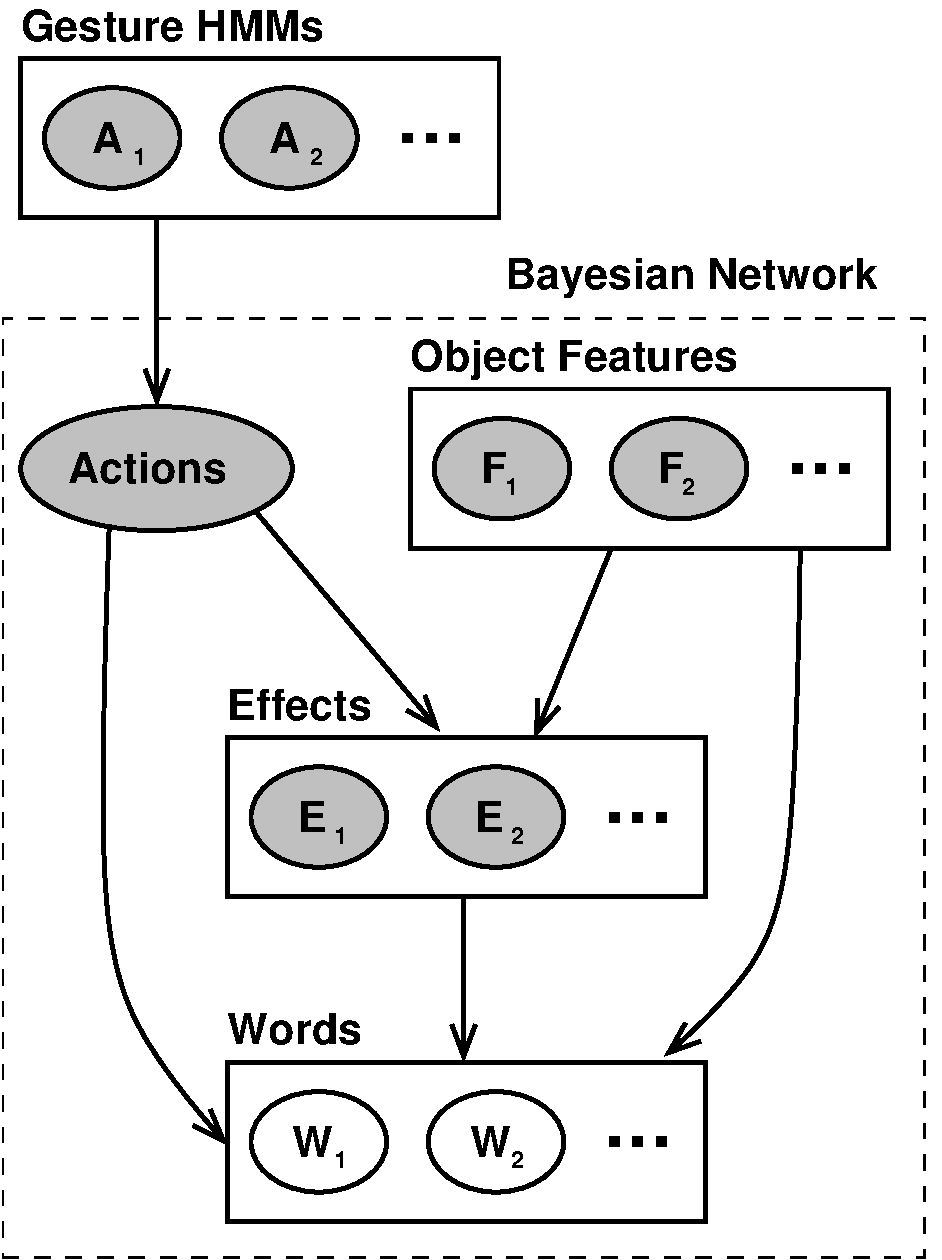
\includegraphics[width=\columnwidth]{fullNetAbstract}
  \caption{Abstract representation of the probabilistic dependencies in the model.}
\end{figure}

In the experimental section, we will show that what the robot has learned subjectively or alone~(by self-exploration, knowing the action identity as a prior~\cite{salvi:2012:smcb}), can subsequently be used when observing a new agent~(human), provided that the actions can be estimated with \acp{HMM} as in~\cite{saponaro:2013:crhri}.

%%%%%%%%%%%%%%%%%%%%%%%%%%%%%%%%%%%%%%%%%%%%%%%%%%%%%%%%%%%%%%%%%%%%%%%%%%%%%%%%
\section{Experimental Results}

\acp{BN} are flexible, they can be used for different purposes

\subsection{Object Shape Estimation}

estimate object shape, based on inferred action (gesture) and resulting effect. $p(O \mid A, E)$

\subsection{Effect Prediction}

$p(E \mid A, O)$


%%%%%%%%%%%%%%%%%%%%%%%%%%%%%%%%%%%%%%%%%%%%%%%%%%%%%%%%%%%%%%%%%%%%%%%%%%%%%%%%
\section{Conclusions and Future Work}

blah

%%%%%%%%%%%%%%%%%%%%%%%%%%%%%%%%%%%%%%%%%%%%%%%%%%%%%%%%%%%%%%%%%%%%%%%%%%%%%%%%
\section{Acknowledgements}
This research was partly supported by the CHIST-ERA project IGLU.
We thank Konstantinos~Theofilis for his software and help permitting the acquisition of human hand coordinates in \hri{} scenarios with the iCub robot.%~(\url{http://wiki.icub.org/wiki/OpenNI2}). % TODO uncomment

%%%%%%%%%%%%%%%%%%%%%%%%%%%%%%%%%%%%%%%%%%%%%%%%%%%%%%%%%%%%%%%%%%%%%%%%%%%%%%%%
%The reference format is the standard IEEE one. References should be numbered in order of appearance
%\newpage
%\balance
\nocite{*} % TODO remove this when article is finished
\bibliographystyle{IEEEtran}
%\bibliographystyle{IEEEtran/bibtex/IEEEtran}
\bibliography{glu2017_bibliography}

\end{document}
